\chapter{Robustness Study Using Monte Carlo Methods}
\label{c:robustness}

Monte Carlo Method explained --> Statisitical Approcach etc.

\section{Definition of Parameter Boundaries}%
\label{c:robustness:s:parameter}

Statistical Exploration of the Data from System Identification!

\section{Robustness of SISO Systems} % (fold)
\label{c:robustness:s:siso}

\begin{figure}[H]
\begin{minipage}[b]{\textwidth}
\centering
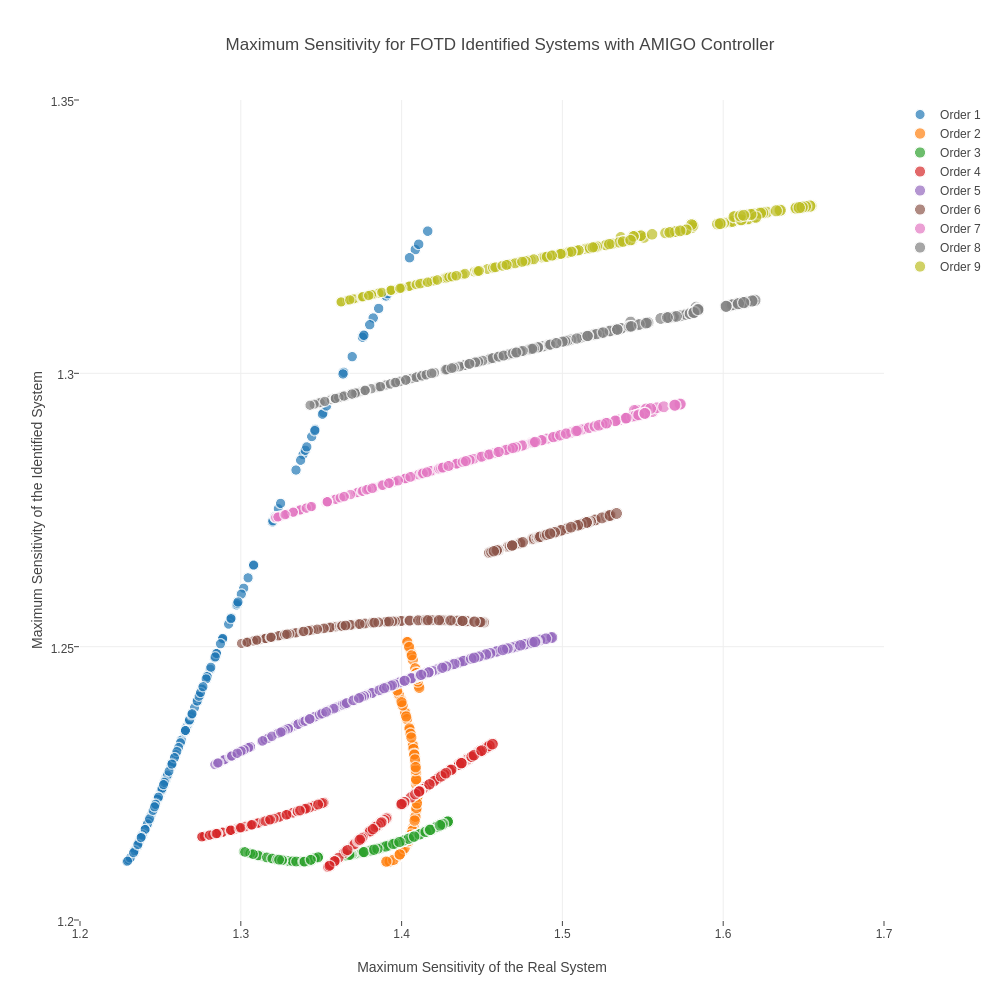
\includegraphics[width=0.9\textwidth]{./Graphics/PT9-Study.png}
\caption{Results of the Robustness Study, Maximum Sensitivity of the Real System and the Identified System}
\label{c:control:f:robustness_study}
\end{minipage}
\end{figure}

\section{Robustness of MIMO Systems}
\label{c:robustness:s:mimo}

\begin{figure}[H]
\begin{minipage}[b]{\textwidth}
\centering
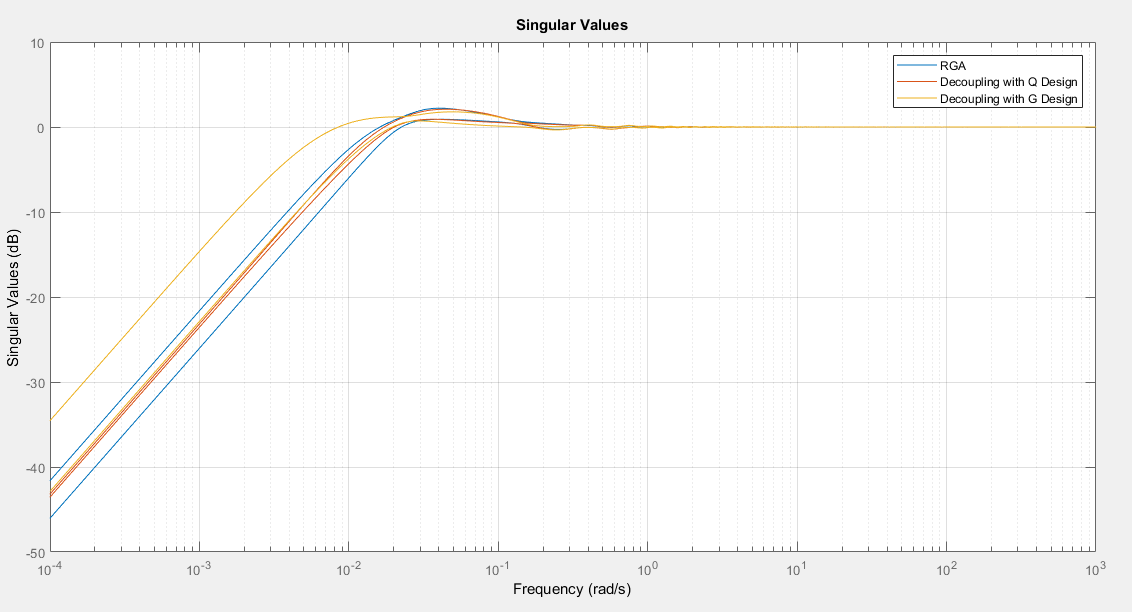
\includegraphics[width=0.9\textwidth]{./Graphics/SVD_MATLAB.png}
\caption{Robusteness of the MIMO}
\label{c:robustness:f:mimo_svd}
\end{minipage}
\end{figure}
